\documentclass{beamer}
\usepackage[utf8]{inputenc}
\usepackage{graphicx}
\usepackage{amsmath}
\usepackage{booktabs}
\usepackage{longtable}

\usetheme{CambridgeUS}

\setbeamertemplate{caption}{\centering\insertcaption\par}

\title{Vektorová reprezentace projektů VaVaI}
\author{Pavel Mikuláš}
\institute[MFF UK]%
{
  \inst{}%
  Matematicko-fyzikální fakulta\\
  Univerzita Karlova
}
\date{Ročníkový projekt, 2019/2020}

\begin{document}

\maketitle

\section{Úvod}


\begin{frame}
\frametitle{Co bylo předmětem zkoumání...}

  \begin{itemize}
    \item Struktura a rozdělení projektů \pause
    \item Minimální popis projektu \pause
    \item Způsoby vektorové reprezentace projektů \pause
    \item Shlukování vektorových reprezentací \pause
    \item Interpretace úvodních pokusů o shlukování
  \end{itemize}

\end{frame}

\section{Data}
\subsection{Struktura a rozdělení projektů}

\begin{frame}
  \frametitle{Popis projektu}

  \begin{figure}[!h]
      \centering
      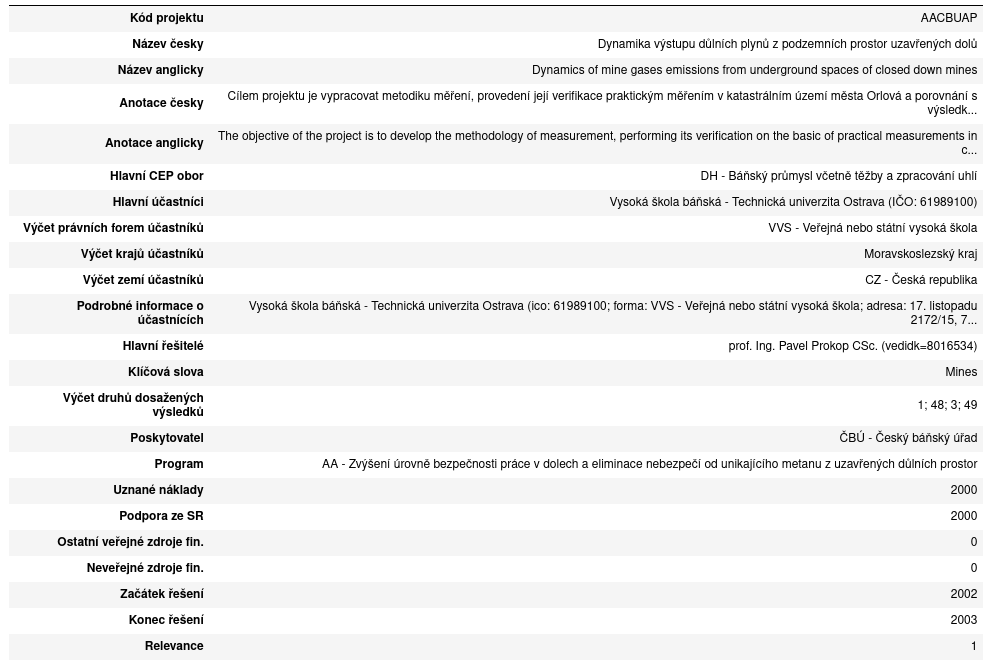
\includegraphics[width=.85\textwidth,height=\textheight,keepaspectratio]{figures/complete_rep.png}
      \label{fig:complete_rep}
  \end{figure}
\end{frame}

\begin{frame}
  \frametitle{Počty projektů podle poskytovatelů}

  \begin{figure}[!h]
      \centering
      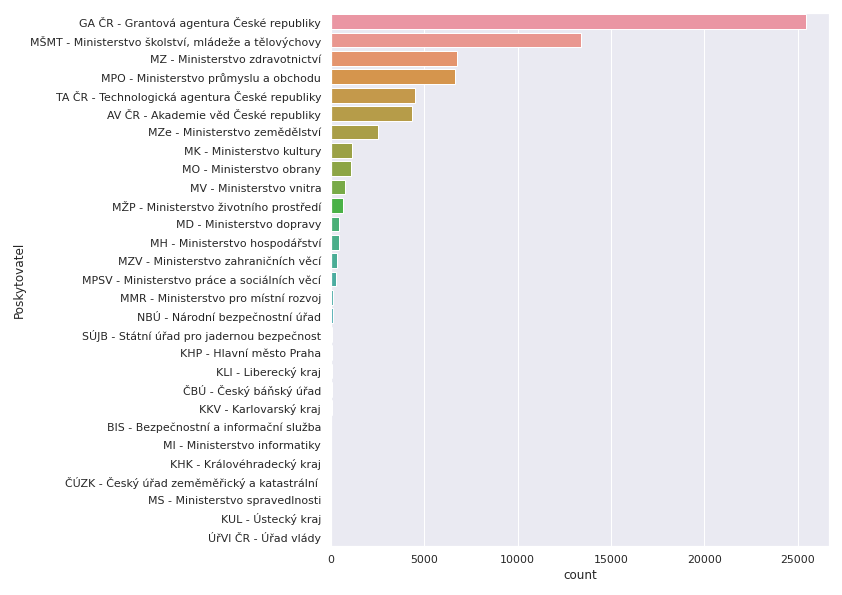
\includegraphics[width=.85\textwidth,height=\textheight,keepaspectratio]{figures/poskytovatele.png}
      \label{fig:poskytovatele}
  \end{figure}

\end{frame}

\begin{frame}
  \frametitle{Počty projektů podle oborů CEP}

  \begin{figure}[!h]
      \centering
      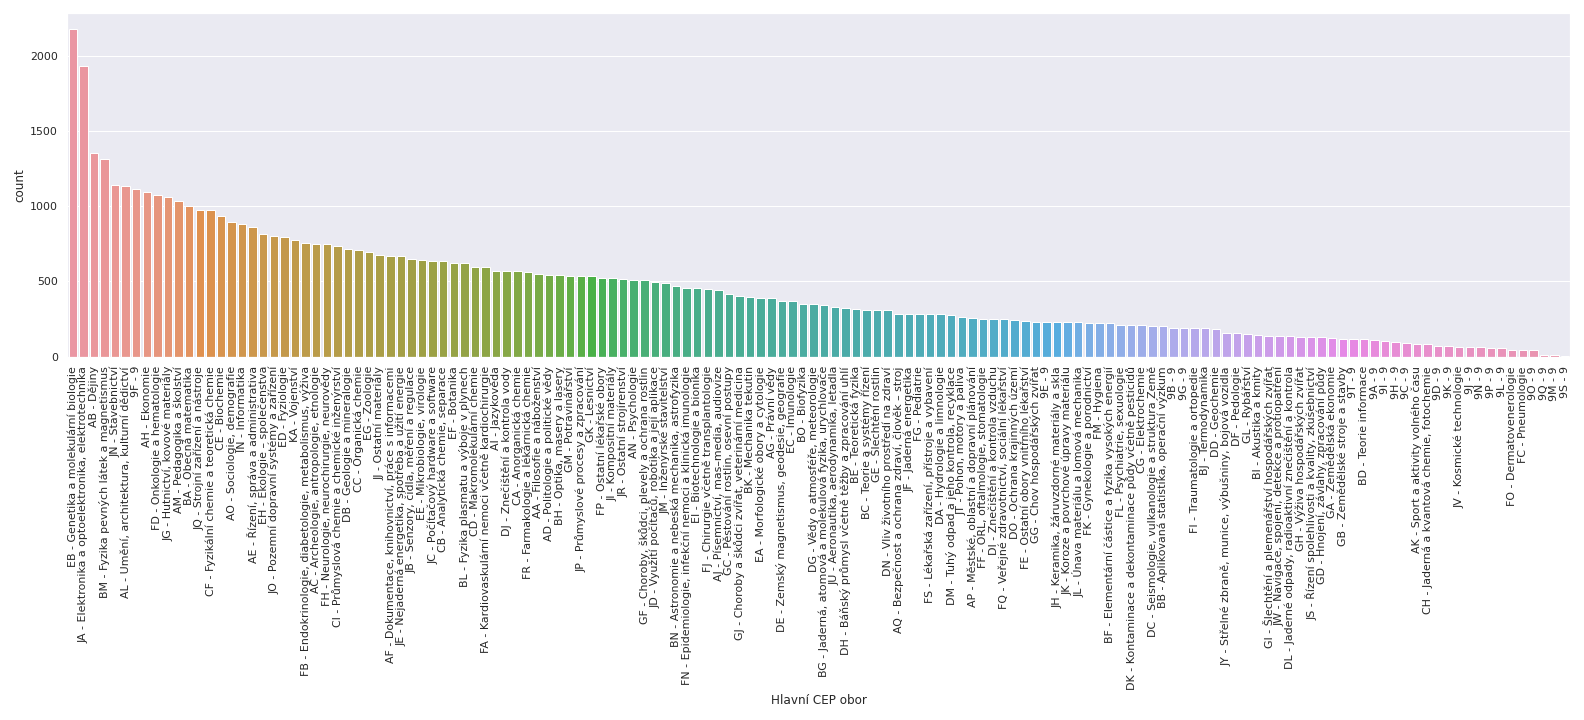
\includegraphics[width=\textwidth,height=\textheight,keepaspectratio]{figures/obory.png}
      \label{fig:obory}
  \end{figure}

\end{frame}


\subsection{Minimální popis projektu}

\begin{frame}
\frametitle{Nevyužité atributy}

  \begin{figure}[!h]
      \centering
      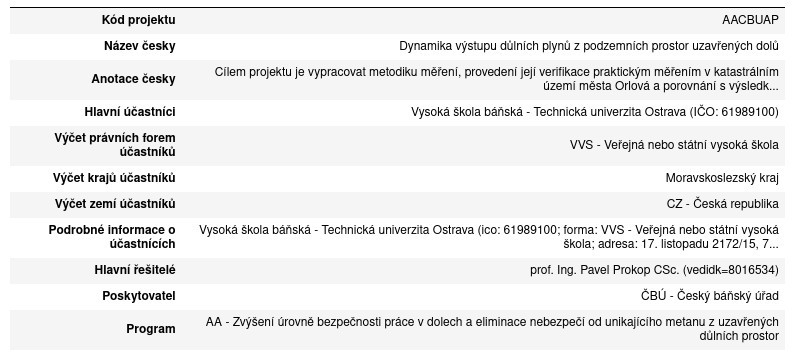
\includegraphics[width=.85\textwidth,height=\textheight,keepaspectratio]{figures/unused.png}
      \label{fig:unused}
  \end{figure}

\end{frame}

\begin{frame}
\frametitle{Atributy použité k reprezentaci projektů}

  \begin{figure}[!h]
      \centering
      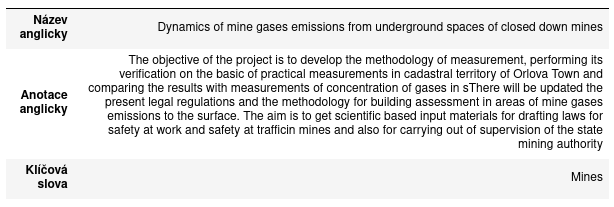
\includegraphics[width=.7\textwidth,height=\textheight,keepaspectratio]{figures/used.png}
      \label{fig:used}
  \end{figure}

\end{frame}

\section{Vektorizace projektů}
\subsection{Lemmatizace}

\begin{frame}
\frametitle{Reprezentace projektu jedním řetězcem}

  \centering
  Zřetězením anglických textů získáme minimální popis projektu pomocí jednoho retězce. \\ \pause
  \vspace*{\fill}
  Řetězec převedeme na malá písmena a odstraníme diakritiku a "stop-words". \\ \pause
  \vspace*{\fill}
  Pro redukci velikosti slovníku tento řetězec následně zlemmatizujeme. \\

\end{frame}

\begin{frame}
\frametitle{Příklad textu před lemmatizací}
  \begin{overprint}
    \onslide<1>\resizebox{.51\textwidth}{!}{\begin{tabular}{l}
\toprule
text \\
\midrule
this sentence is about whales \\
this sentence is about kangaroos \\
this sentence is about rhinos \\
this is an another sentence about whales \\
yet another sentence about kangaroos \\
\bottomrule
\end{tabular}
}
    \onslide<2>\resizebox{\textwidth}{!}{\begin{tabular}{ll}
\toprule
                                     text &                          text\_lemmatized \\
\midrule
            this sentence is about whales &             this sentence is about whale \\
         this sentence is about kangaroos &          this sentence is about kangaroo \\
            this sentence is about rhinos &             this sentence is about rhino \\
 this is an another sentence about whales &  this is an another sentence about whale \\
     yet another sentence about kangaroos &      yet another sentence about kangaroo \\
\bottomrule
\end{tabular}
}
  \end{overprint}
\end{frame}


\subsection{Vektorizace}

\begin{frame}
\frametitle{TF-IDF}

\begin{columns}
  \column{.5\textwidth}
    \begin{overprint}
      \onslide<1>\centering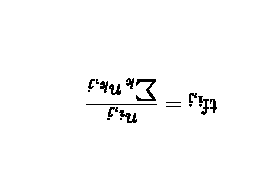
\includegraphics[width=.6\textwidth,height=\textheight,angle=180,keepaspectratio]{figures/tf.pdf}
      \onslide<2->\centering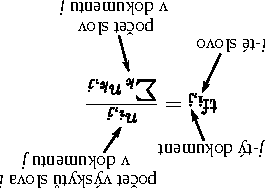
\includegraphics[width=.6\textwidth,height=\textheight,angle=180,keepaspectratio]{figures/tf_described.pdf}
    \end{overprint}

  \column{.5\textwidth}
    \begin{overprint}
      \onslide<1-2>\centering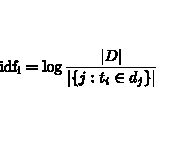
\includegraphics[width=.5\textwidth,height=\textheight,keepaspectratio]{figures/idf.pdf}
      \onslide<3->\centering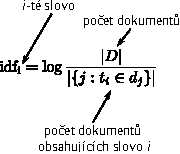
\includegraphics[width=.5\textwidth,height=\textheight,keepaspectratio]{figures/idf_described.pdf}
    \end{overprint}
\end{columns}

\end{frame}

\begin{frame}
\frametitle{TF-IDF}

  \vspace{20pt}
  \begin{overprint}
    \onslide<1-2>\centering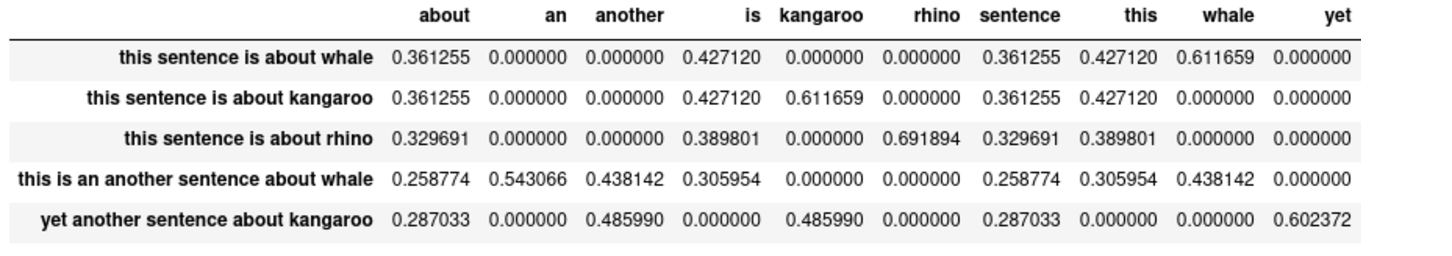
\includegraphics[width=\textwidth,height=\textheight,keepaspectratio]{figures/whale_vectorized.pdf}
    \onslide<3>\centering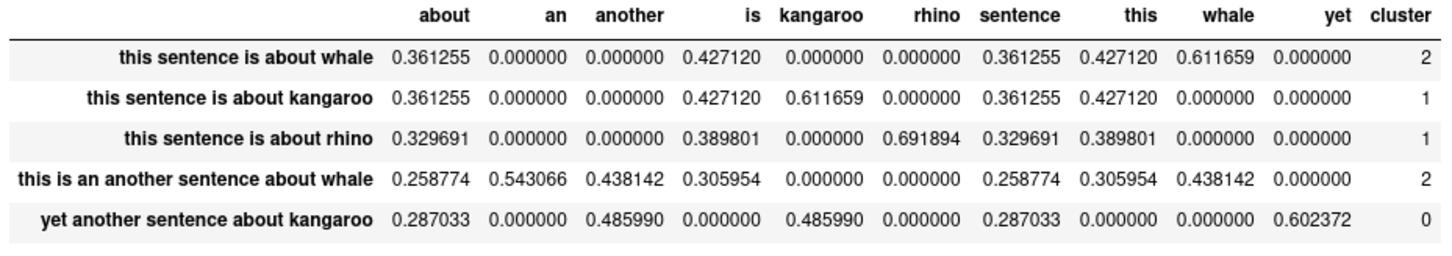
\includegraphics[width=\textwidth,height=\textheight,keepaspectratio]{figures/whale_vectorized_clust.pdf}
  \end{overprint}
  \vspace{20pt}
  \begin{overprint}
    \onslide<2>\centering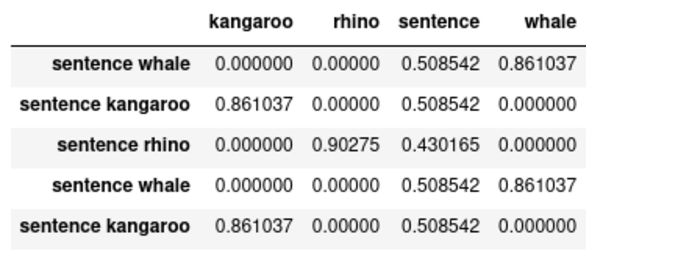
\includegraphics[width=.5\textwidth,height=\textheight,keepaspectratio]{figures/whale_stopwords.pdf}
    \onslide<3>\centering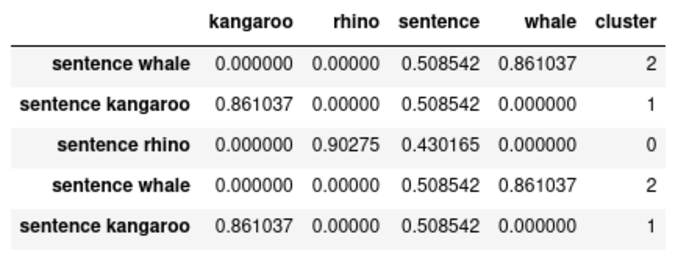
\includegraphics[width=.5\textwidth,height=\textheight,keepaspectratio]{figures/whale_stopwords_clust.pdf}
  \end{overprint}

\end{frame}


\subsection{Clustering}
\begin{frame}
\frametitle{Elbow method}

  \vspace{10pt}
  \begin{figure}[t]
      \centering
      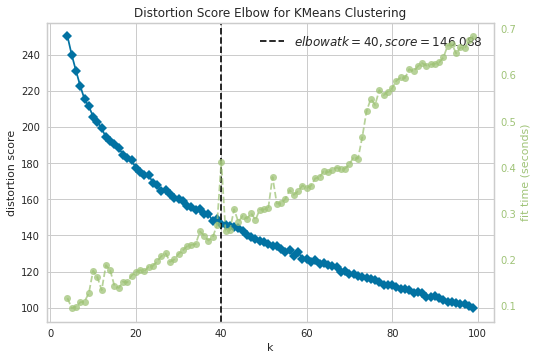
\includegraphics[width=.6\textwidth,height=\textheight,keepaspectratio]{figures/elbow.png}
      \label{fig:used}
  \end{figure}
\end{frame}

\begin{frame}
  \frametitle{t-SNE}

  \begin{figure}[t]
      \centering
      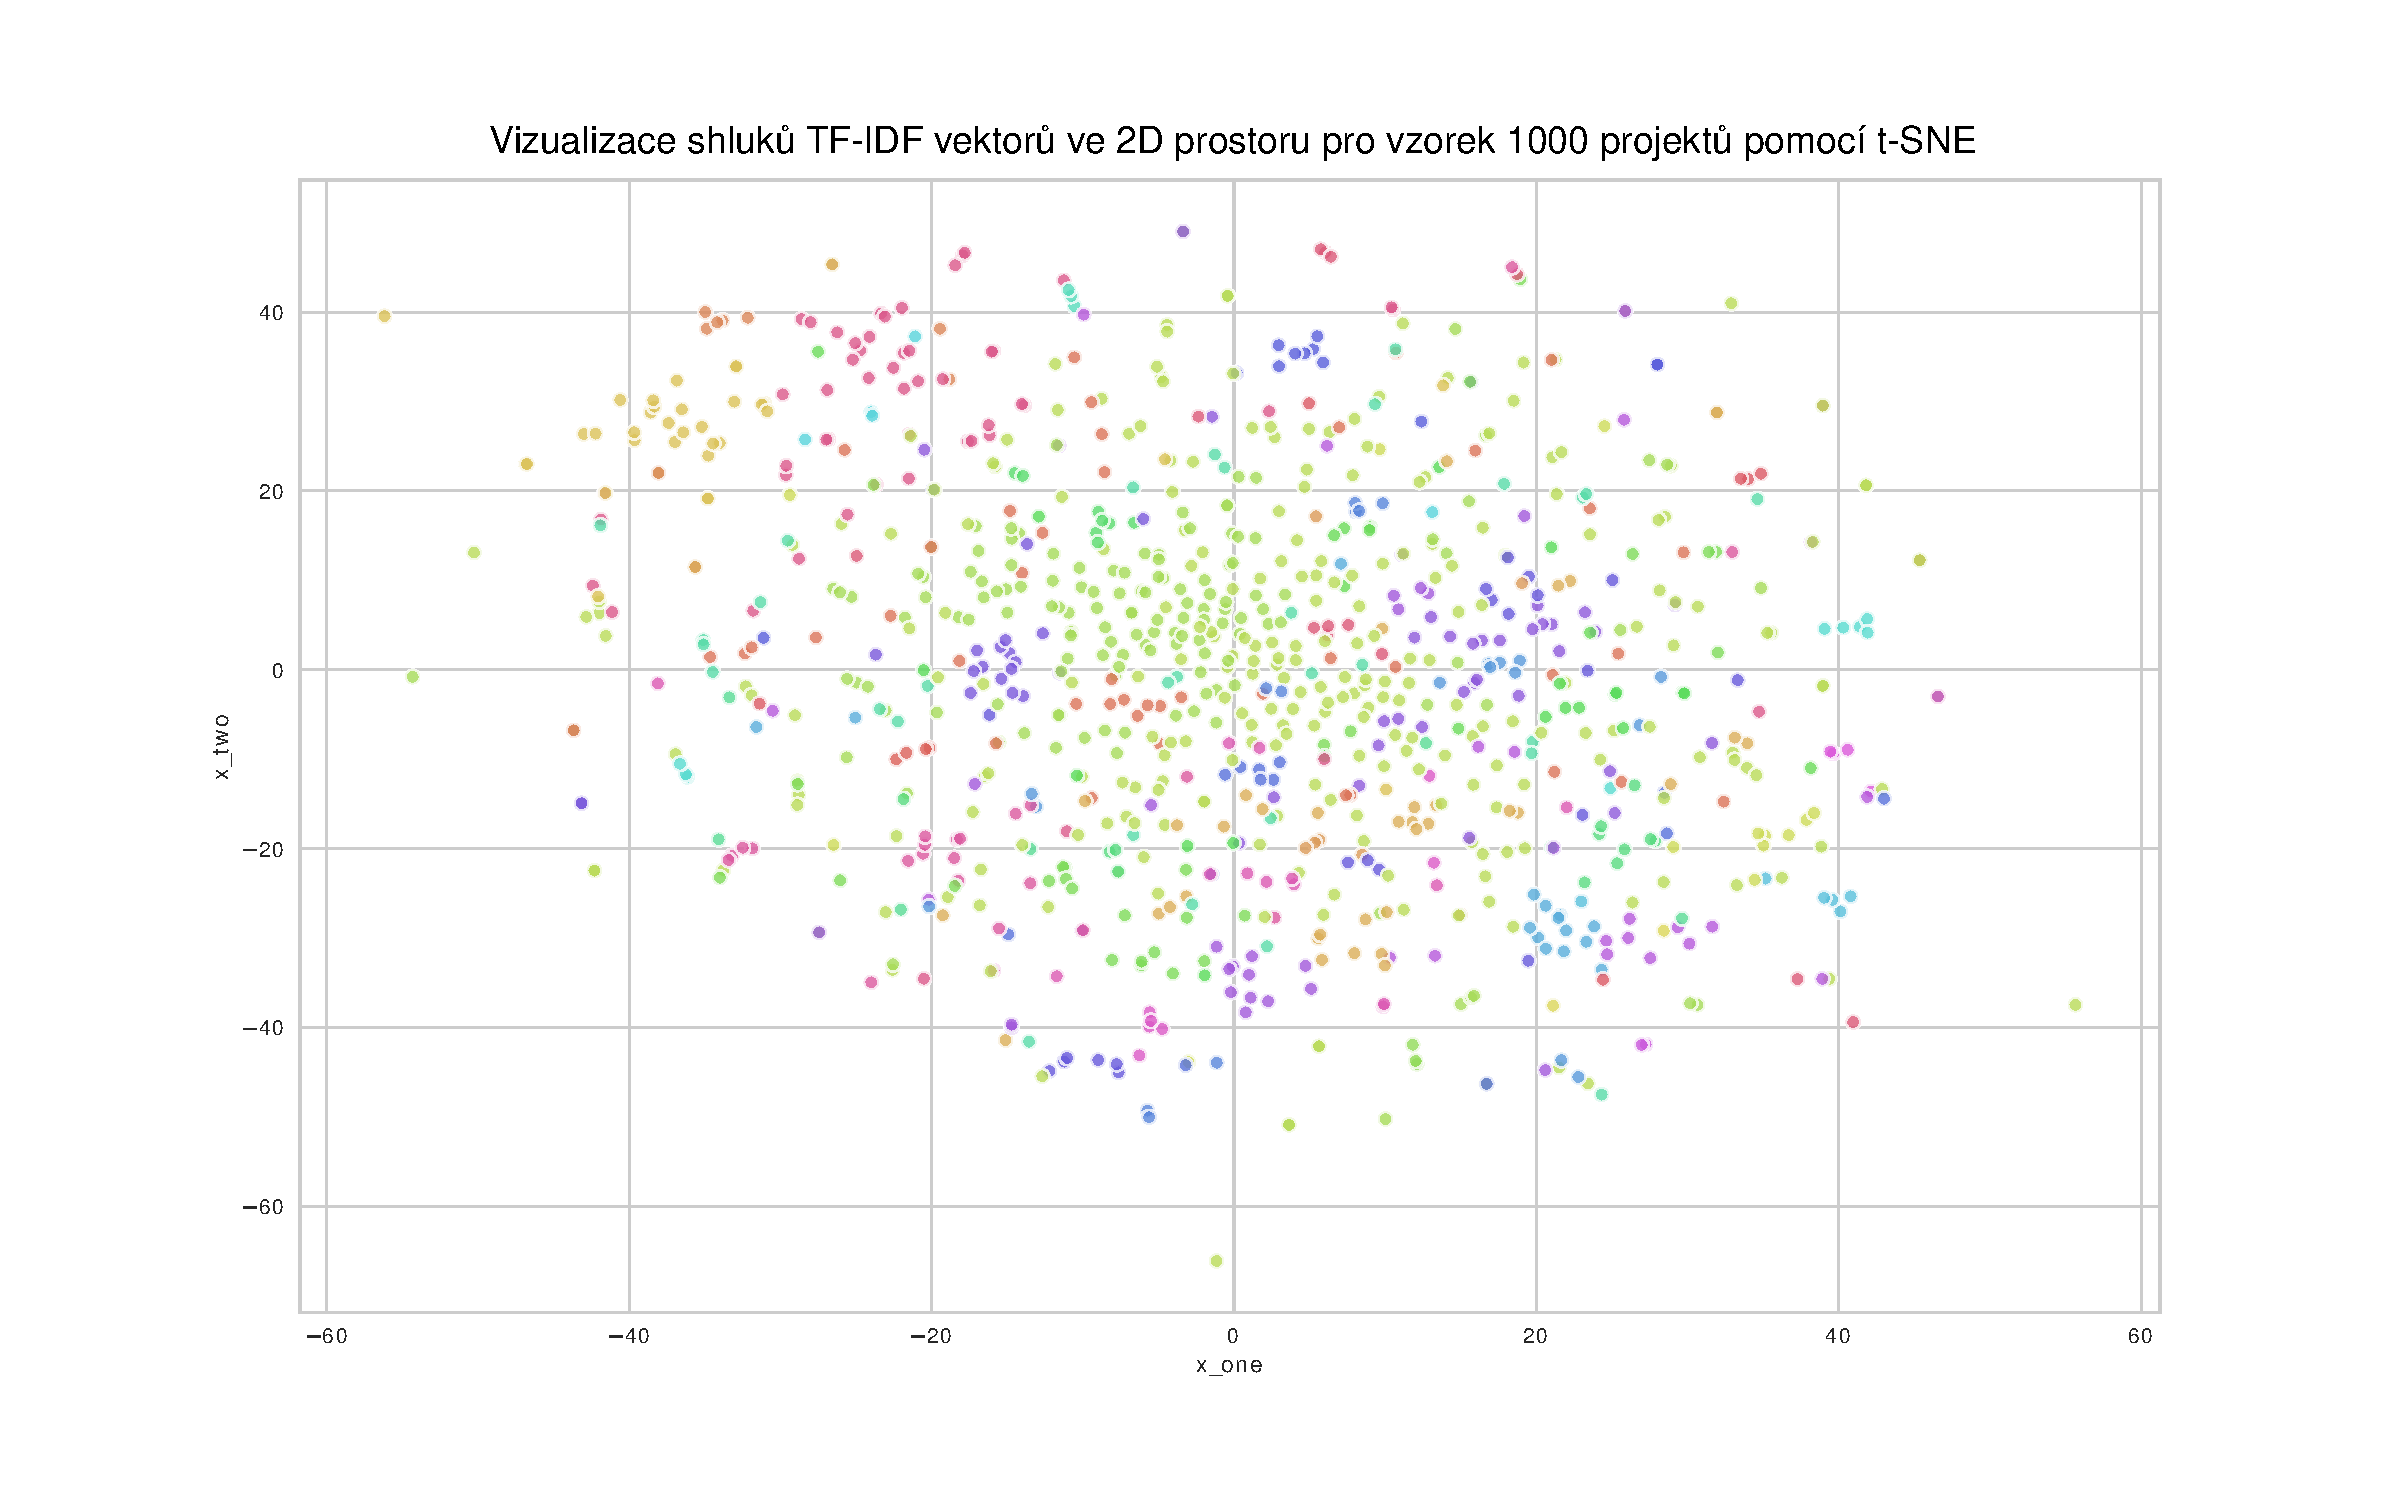
\includegraphics[width=\textwidth,height=\textheight,keepaspectratio]{figures/tfidf_tsne.pdf}
      \label{fig:used}
  \end{figure}
\end{frame}

\begin{frame}
\frametitle{word2vec}

  \begin{figure}[t]
      \centering
      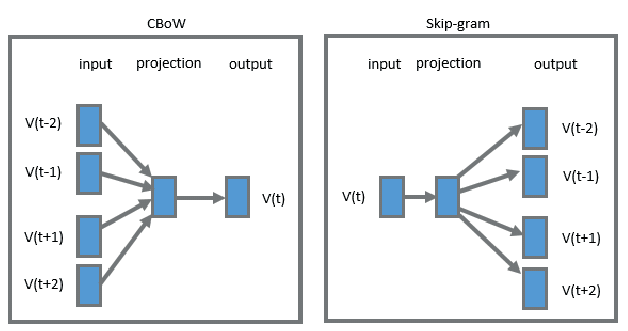
\includegraphics[width=0.7\textwidth,height=\textheight,keepaspectratio]{figures/word2vec_diagram.png}
      \caption{Schéma word2vec modelu {\tiny (10.1109/UBMK.2017.8093492.)}}
      \label{fig:used}
  \end{figure}

\end{frame}


\begin{frame}
\frametitle{word2vec}

  \begin{figure}[t]
      \centering
      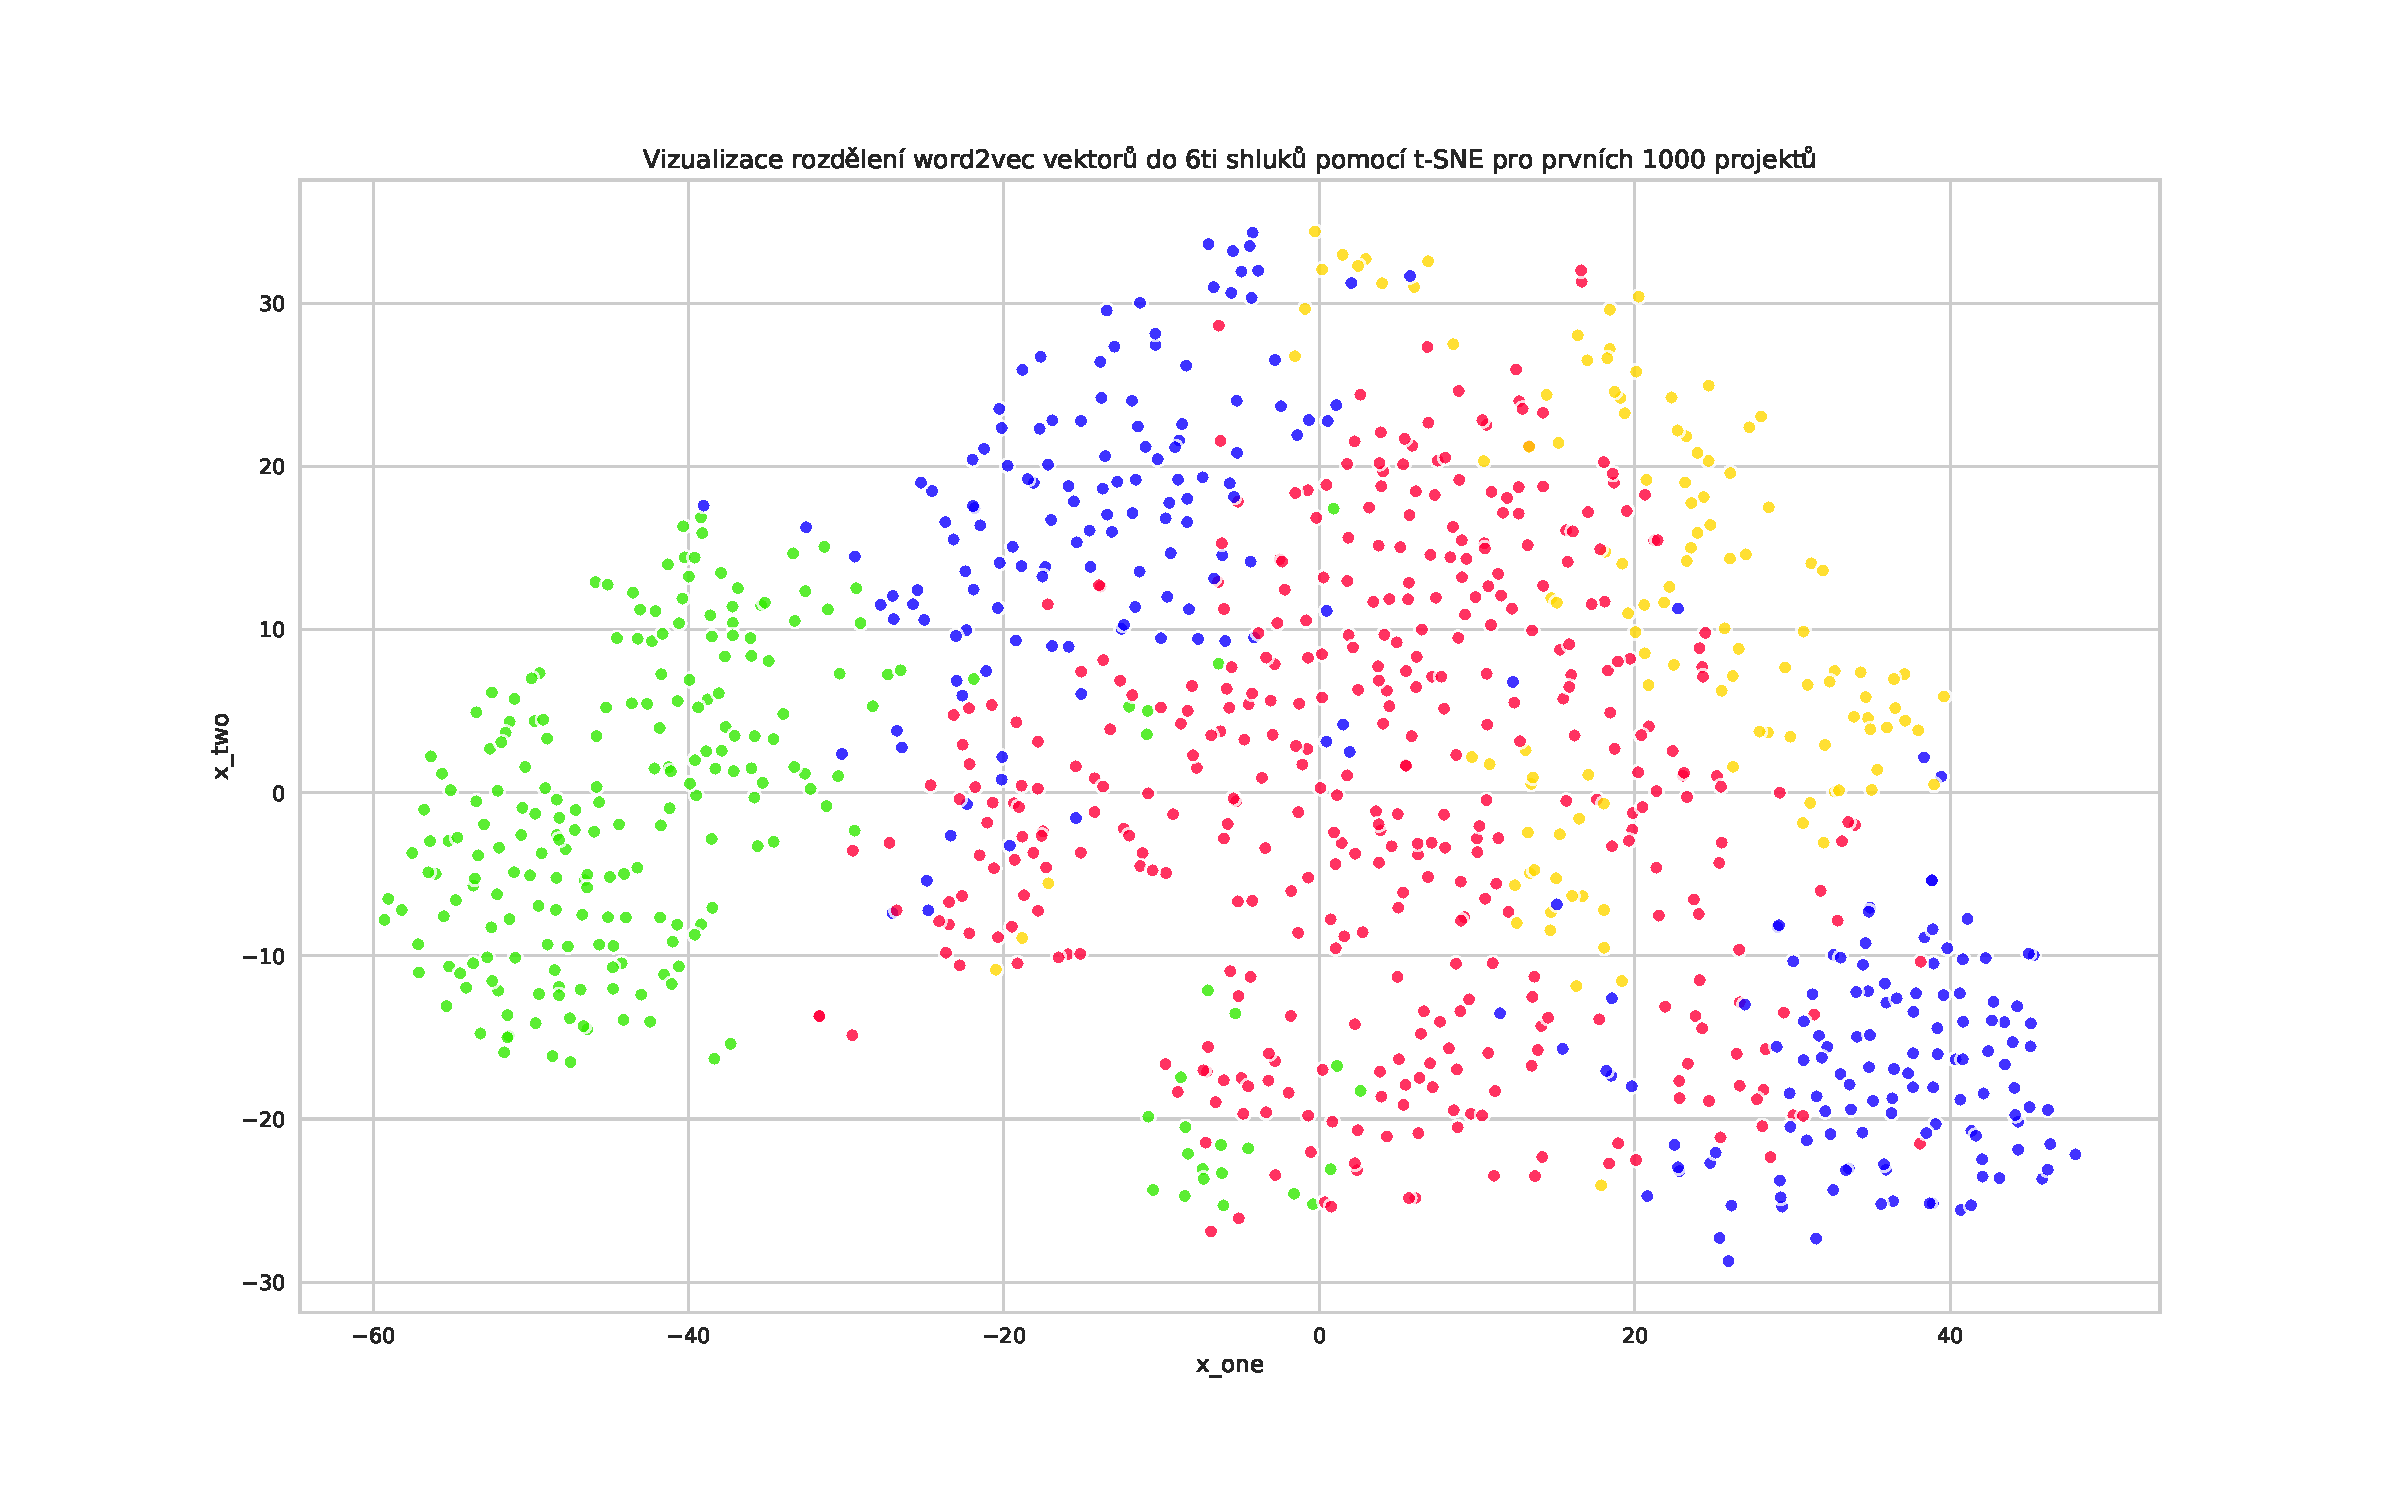
\includegraphics[width=\textwidth,height=\textheight,keepaspectratio]{figures/word2vec_tsne.pdf}
      \label{fig:used}
  \end{figure}

\end{frame}
\end{document}
